\input{chapter-header.tex}
% ===========================================================================
\chapter{State of the Art}
\chaplabel{background}
\minitoc
% ===========================================================================
\introduction
% ===========================================================================
	
	
% ===========================================================================
\newpage
% ===========================================================================
\section{On Evolving a Language Kernel}

The evolution of a language kernel presents two main challenges to solve: changing the elements of compliance with its Virtual Machine and changing elements having an impact on the system's meta-circularities.

\subsection{Changing the Language-VM Interface}

\gp{maybe this first part explaining problems could be part of the problem statement in the introduction}
%\gp{not sure if defining metacircularities is useful}The causal connections define circular definitions in the system, namely \emph{metacircularities}~\cite{Chib96a, Denk08b}.
Modifying a language kernel to adapt it to these and other situations~(either to do bug fixing or add new features to it) becomes a cumbersome task for some of the following reasons: 
\begin{description}
\item[High amount of low level code.] The initialization of the language's circular definitions is often done in the VM by using a low level language, often a mixture of C, C++ and Assembly. This poses a high entry barrier to developers not versed in such kind of languages.
\item[Language definition is scattered.] The language kernel under initialization is defined by both source code files written in the same language and imperative code present in the VM. Although splitted and scattered, they define the same language and a change in one of these parts may impact on the other one.
\item[Runtime initialization mixes concerns.] The initialization of the language kernel is mixed ~(and coupled) with the initialization of the rest of the runtime system. This introduces an undesired coupling that affects the development and the understanding of the code.
\end{description}

\gp{write the related work of the new bootstrap paper: metacircular vas help to solve the gap between the language kernel and the VM, and so, easing the change of interface. See Jikes RVM, SqueakVM, Klein VM allow some grade of bootstrap or manipulation of the underlying runtime system}

\subsection{Changing a Language's Metacircularities}

Some methods or classes in a Smalltalk image are very sensitive to changes, either because they are used pervasively throughout the system, or take part in important subsystems like the user interface, the compiler, the debugger, the metaclass hierarchy, or classes that are well-known to the virtual machine.
This is because Smalltalk has a single scope where not only everything is visible, but also reflectively accessible.
Any breakage in this kind of code usually leads to spectacular failure. A simple example would be adding a breakpoint in the iterator method \ct{Array>>do:}. In Pharo Smalltalk, adding this breakpoint impacts about 90000 \ct{Array} instances and the image freezes \cite{Denk08b}.
It is thus very difficult to debug or change this code in a realistic setting, without risking to impact the whole image.

But the fact is, some evolutions do require changes to this sensitive code.
If temporary breakage is necessary, then the maintainers must find a way to apply the changes with reduced tools and extra care.
Alternatively, some images are destined to run under restricted conditions that make it impractical to include a complete set of development tools, or simply to access them: for instance, images running on remote servers do not have an active graphical interface\footnote{Remote display solutions like VNC do exist, but suffer from usability and portability problems.}.
This makes development, testing, and maintenance impractical or even impossible.

Current solutions or workarounds are to work on a renamed copy of the classes, or to remotely control a separate image via remote objects.
However, in the first case we only delay the problem, because the complete impact of changes cannot be assessed until the copied and modified classes are merged back into the system.
In the latter case, if a change causes the remote image to crash, then it will be impossible to assess the problem.

The most related family of work is virtualization approaches like Xen \cite{Chis07xen}. Virtualization makes it possible to run several operating systems at once on a single physical machine. As these approaches target full operating systems, they rely on support from the hardware platform, and in some cases from the guest OS; they also concentrate on performance and production features, and consider the guest system mostly as a black box. In contrast, ObjectSpaces provide full control and reflective access to their contents.

Changeboxes \cite{Denk07c} encapsulate and scope changes, allowing several versions of a system to coexist in a single runtime environment, effectively adapting version control from static source code to running systems. Changeboxes scope code changes, while ObjectSpaces scope generic object references; also, Changeboxes do not directly address the problem of applying changes to code that is critical to the runtime system itself.

Scoping side-effects has been the focus of two recents works. Worlds~\cite{Wart08a} provide a way to control and scope side-effects in Javascript. Similar to
ObjectSpaces, side-effects are limited to a first-class environment.  Tanter proposed a more flexible scheme: contextual values~\cite{Tant08b} are scoped 
by a very general context function.

One problem meta-circular architectures is that meta-objects rely on the same code they reflect upon; therefore there is a risk of infinite meta-recursion when the meta-level instruments code that it relies upon.
In \cite{Denk08b}, Denker et al solve this problem by tracking the degree of metaness of the execution context. Meta-objects can only reflect on objects of a lower metaness, thus simulating the semantics of an infinite tower of distinct meta-interpreters. The existing work on Meta-context is only concerned with scoping behavioral changes. More work is needed to extend this work to structure. We plan to explore how ObjectSpaces can be used to provide a way to control structural reflective change.

One possibility for implementing ObjectSpaces is to differentiate messages depending on whether the sender and the receiver are in the same space or not. Several works use a similarly extended message lookup.
%
Us~\cite{Smit96a} is a system based on Self that supports subject-oriented
programming~\cite{Harr93a}. Message lookup depends not only on the receiver of a
message, but also on a second object, called the \emph{perspective}.
The perspective allows for layer activation.
ContextL~\cite{Cost05a, Hirs08a} is a language to support Context-Oriented 
Programming (COP). The language provides a notion of \emph{layers}, which
package context-dependent behavioural variations. In practice, the variations
consist of method definitions, mixins and \emph{before} and \emph{after}
specifications. Layers are dynamically enabled or disabled based on the current
execution context. ObjectSpaces provide form a context. The relationship between
context-oriented programming, subjectivity and ObjectSpaces is an interesting
topic of future research.

Gemstone \cite{Otis91a} provides the concept of class versions. Classes are
automatically versioned, but existing instances keep the class (shape and
behavior) of the original definition. Instances can be migrated at any time.
Gemstone provides (database) transaction semantics, thus state can be rolled
back should the migration fail.
Gemstone's class versions extend the usual Smalltalk class evolution mechanism for robustness, 
large datasets, and domain-specific migration policies. In contrast, ObjectSpaces target general 
reflective access and bootstrap-like evolutions of code that is critical to the environment.

In Java, new class definitions can be loaded using a class loader
\cite{Lian98a}. Class loaders define namespaces, a class type is defined by the
name of the class and its class loader. Thus the type system will prohibit
references between namespaces defined by two different loaders. Class loaders
can be used to load new versions of code and allow for these versions to coexist
at runtime, but they do not provide a first-class model of change.
Java also provides JPDA, a remote debugging architecture that specifies a native interface on the debuggee VM, and a matching API for the debugger front-end, running in a separate VM. However, JDPA only supports introspection features like  inspection and monitoring, and very limited intercession \cite{jdpa}.


\section{On Evolving Applications}

 \begin{table*}[ht]
 \small
 	\centering
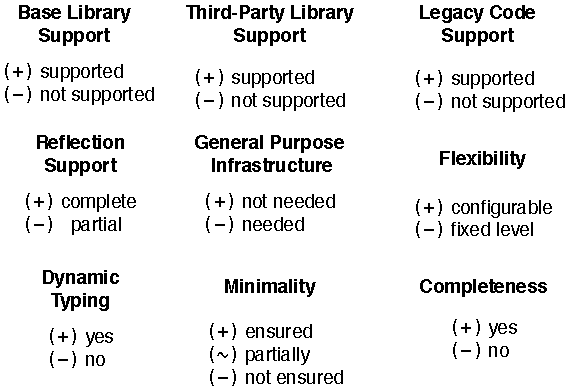
\includegraphics[width=\linewidth]{criteria_overview}
 	\begin{tabular}{|ccccc>{\columncolor[gray]{0.8}}c|}
	
\hline
 			& \textbf{Dedicated}
 			& \textbf{Static}
			& \textbf{Hybrid}
 			& \textbf{Dynamic}
 			& \textbf{Tornado} \\
 			& \textbf{SDKs}
 			& \textbf{Analysis}
			& \textbf{Analysis}
 			& \textbf{Analysis}
 			& \\
%  \cmidrule(r){2-6}
% \midrule

		Base Library&&&&&\\Support
 			& + & + & + & + & +\\
		\hline
		Third-Party&&&&&\\ Library Support
 			& - & + & + & + & +\\
		\hline
		Legacy Code&&&&&\\ Support
 			& - & + & + & + & + \\
		\hline
		Reflection&&&&&\\ Support
 			& + & - & - & + & + \\
		\hline
		Special&&&&&\\ Infrastructure& - & + & - & - & + \\for Running
 			&&&&&\\
		\hline
		Flexibility
 			& - & - & - & - & +  \\
 	 \hline
 	\end{tabular}
 	\caption{Evaluation criteria applied to related work on deployment code unit tailoring techniques}
 	\label{tb:comparison}
 \end{table*}
 
The reduction of the deployment footprint of object-oriented applications has been subject of interest both in industry and research since many years. In such regard, we identified four different families of solutions for dead code elimination: dedicated SDKs~(cf. section \ref{section:static_selection_rw}), static analyses~(cf. section \ref{section:static_rw}), dynamic analyses~(cf. section \ref{section:dynamic_rw}) and hybrid analyses~(cf. section \ref{section:hybrid_rw}). Table~\ref{tb:comparison} presents a comparison of these techniques, given the criteria defined in section~\ref{sec:criteria}.

\subsection{Dedicated SDKs}%Pre-conceived specialized application-independent platforms}
\label{section:static_selection_rw}

Dedicated SDKs are SDKs containing frameworks and/or libraries prepared to run under specific circumstances. For example, Java Micro Edition~(J2ME)~\cite{JavaME} as the dedicated version of the Java SDK, or Cocoa Touch as the one of Cocoa. These specialized SDKs are reduced platforms to run applications inside mobile and constrained devices. These platforms provide a reduced and fixed set of base libraries defined a priori and in a not customizable way. Applications have to be written especially for them, and thus legacy code and third-party libraries not written especially for it are not compatible. Reflection is available since the statically tailored base libraries are built in a not automatic fashion, and the application code is not tailored.

\subsection{Static Analysis-Based Techniques}\label{section:static_rw}

Static analysis approaches for dead code elimination make use of the static information of a program to select the minimal subset of used elements. The bibliography describes four different algorithms to achieve this goal: unique name, class hierarchy analysis~(CHA), rapid type analysis~(RTA) and reachable members analysis~(RMA) \cite{Baco96a, Titz06a}. These techniques share a common approach, selecting an entry point method of an application and following from it the execution flow using the available static information \ie type annotations, and class and method names, building a call-graph~\cite{ShortGrov97a}.

These techniques have been studied and applied in many environments and languages. Rayside et al.~\cite{ShortRays02a}, Jax~\cite{ShortTip03a} and the ExoVM System~\cite{Titz06a} propose application extraction tools using these techniques for Java applications. Sallenave et al.~\cite{Sall10a} apply RTA to produce smaller .NET assemblies for embedded systems. Bournoutian et al.~\cite{Bour14a} use CHA to optimize on-device Objective-C applications.

In summary, these approaches are based on the static types found either in the source code or byte code. Thus, they are not applicable efficiently in dynamic languages with no static type information. These solutions are valuable as they allow one to tailor base and third-party libraries, and legacy code. Their tailoring approach generates new deployment units that can run on the standard runtime infrastructure. The main drawback of this approach appears in the presence of reflection and configuration files, which will only work with a subset of reflective invocations through complementary analyses on the strings found in the source code. Also, existing solutions in this family lack the flexibility to declare and identify levels of tailoring, making it an "all or nothing".

\gp{Closed World Assumption kills you guys!}

\subsection{Dynamic Analysis-Based Techniques}\label{section:dynamic_rw}

Dynamic analysis techniques use exclusively runtime information~(\ie execution flow, alive objects, execution statistics) to perform dead code elimination. Amongst these, we identify two different approaches: \emph{load on demand} and \emph{code collection}. Load on demand approaches detect during runtime whenever a class or method needs to be installed and request it to a server application. Code collection approaches deploy the full application  and garbage collect unused code based on usage statistics. Related work in this family share a common characteristic: these techniques are used inside ubiquitous systems \ie systems meant to be always connected. Ubiquitous systems, as they are always connected, have a possibility to fallback and recover in the case of incompleteness. However, to focus here on the dead code elimination techniques, we will discuss the incompleteness recovery techniques in section \ref{section:completeness}.

JUCE~\cite{ShortPopa04a,ShortTeod01a} is a platform for ubiquitous devices supporting code load on demand and code collection. Its approach for building up an application is similar to Tornado's. First, it initializes a minimal running application and code is loaded, with a method granularity, from a server located in a different machine. Unused code is collected following usage statistics, and loaded back again on demand if needed.

OLIE~\cite{Gu03a} is an engine that intelligently partitions and offloads objects during runtime to minimize memory consumption. It is part of the adaptive infrastructure for distributed loading (AIDE). In OLIE, offloaded objects are indeed migrated to nearby remote devices. Migrated objects can be accesses later through proxies that perform remote invocations on them.

SlimVM~\cite{Kers09a, Wagn11a} is an ubiquitous system where all code resides on a remote server and is loaded only on demand on small devices. Some static analysis is performed only on the server to reduce the size of the transported code, by identifying most likely needed code. SlimVM changes the class format,  However, on the client side, every code load is done dynamically.

All solutions inside this category share one main property: they require to run the application inside a special infrastructure to apply their techniques \eg specialized VMs implementing remote lazy loading, code collection or special bytecode sets. The main challenge of these solutions resides on applying these techniques while minimizing their impact on performance during the runtime. Additionally, these solutions require their applications to run exclusively inside their infrastructure. Tornado works in the same way as these solutions: it uses a special infrastructure to run the desired application and select the used elements.  However, Tornado provides also with the ability to extract this application and run in \emph{offline} mode, using the non-modified infrastructure.

Regarding dynamic features such as reflection, this kind of solutions are the ones that can, potentially, handle it in the best way since they have in runtime all the information needed to resolve it. JUCE and OLIE, as Tornado, handle naturally reflection as they do not change the runtime representation (which programs make assumptions of, when they use metaprogramming). SlimVM on the other side, had to change the reflection support because they changed the object and class representation on their VM.

Regarding its applicability, SlimVM needs to recompile the whole application into its own format, while OLIE and JUCE, as Tornado, can tailor base and third party libraries without any modifications on it. Thus, the latter two can be applied to legacy code also for free. None of these solutions provide with the ability to select the level of tailoring always working on the full application. In contrast, Tornado uses Seeds to force a minimal subset of elements to be part of the application.


\subsection{Hybrid Analysis-Based Techniques}\label{section:hybrid_rw}

Hybrid analysis techniques mix static and dynamic~(\ie runtime) information to provide better results. The common approach of these is to start an application, such as Tornado does, and pause it after some minimal runtime information is available \ie call stacks are created, some classes are loaded and initialized, and some objects are instantiated. Then, it uses the built stack of alive objects to perform a static analysis, as described in section \ref{section:static_rw}, with concrete type information.

Java in The Small (JITS)~\cite{ShortCour10a} uses a hybrid approach to select the used parts of a program, and then loads them inside a binary image. A specialized VM loads the binary image at startup. JITS's approach tailors base and third-party libraries as well as application specific code. It does not require modifications on the existent application to tailor it, so a legacy application could theoretically be tailored with this approach. JITS does not offer the possibility to configure the tailoring level, since it was designed to be used only in embedded devices where no more than one application would be running. Regarding reflection, JITS presents the same drawbacks as the other static call graph analysis approaches since not all the runtime information about the reflective invocations can be deduced.

% ===========================================================================
\section{Summary and Outlook}
% ===========================================================================


% =============================================================================
\input{chapter-footer.tex}